%-------------------------------------------------------------------------------
\subsection{Modèle d'apparition de tumeurs}
%-------------------------------------------------------------------------------

% Inspiré du modèle d'apparition des tumeurs CDH1 de type II, avec A. Bonnet
% https://www.overleaf.com/project/61fa6f1f2e1b2e66da2e825b
% Transféré dans /home/robin/Bureau/RECHERCHE/GENETIQUE/CDH1/Doc/CDH1_Poisson
% ATTENTION : chgt de notation ! \pi(t) -> 1 - \pi(t).

\paragraph{Modèle.}
On considère l'apparition de tumeurs malignes en deux étapes:
\begin{enumerate}
  \item les tumeurs de type B (bénignes) apparaissent selon un processus de Poisson homogène d'intensité constante $\lambda$ et
  \item chaque tumeur de type B se transforme ensuite en une tumeur de type M (maligne) au bout d'un temps exponentiel de paramètre $\mu$ (donc d'espérance $1/\mu$).
\end{enumerate}

On note $N(t)$ le nombre total de tumeurs apparues au temps $t$ : 
$$
\{N(t)\}_{t \geq 0} \sim PP(\lambda t).
$$
et $M(t)$ le nombre de tumeurs de type M au temps $t$. Le nombre de tumeurs bénignes au temps $t$ vaut donc $B(t) = N(t) - M(t)$.

\bigskip
\paragraph{Question préliminaire.}
\begin{enumerate}
  \item Montrer que si $X$ suit une loi de Poisson $\Pcal(\alpha)$ et que $Y$ sachant $X=x$ suit un loi binomiale $\Bcal(x, p)$, alors $Y$ suit une loi de Poisson $\Pcal(\alpha p)$.
  \solution{
  On intègre la loi conditionnelle de $Y \mid X$ par rapport à la loi de $X$, soit : 
  \begin{align*}
    \Pr\{Y = y\}
    & 
    = \sum_{x \geq y} \Pr\{Y = y \mid X = x\} \Pr\{X = x\}
    = \sum_{x \geq y} \left(\begin{array}{c}x \\ y \end{array}\right) p^y (1-p)^{x-y}e^{-\alpha} \frac{\alpha^x}{x !} \\
    &
    = e^{-\alpha} \sum_{x \geq y} \left(\begin{array}{c}x \\ y \end{array}\right) (\alpha p)^y (\alpha - p)^{x-y} {x !} 
    = e^{-\alpha} \frac{(\alpha p)^y}{y !} \sum_{x \geq y} \frac1{(x - y) !}(\alpha - \alpha p)^{x-y}. 
  \end{align*}
  En posant $z = x-y$, on reconnaît
  $$
  \sum_{x \geq y} \frac1{(x - y) !} (\alpha - \alpha p)^{x-y} 
  =
  \sum_{z \geq 0} \frac1{z !}(\alpha - \alpha p)^{z} 
  =
  e^{\alpha p - \alpha},
  $$
  soit finalement
  $$
  \Pr\{Y = y\}
  = e^{-\alpha} \frac{(\alpha p)^y}{y !} e^{\alpha p - \alpha}
  = e^{-\alpha p} \frac{(\alpha p)^y}{y !}
  $$
  où on reconnaît la loi de Poisson $\Pcal(\alpha p)$. 
  \paragraph{\sl Alternative.} On peut aussi se souvenir que la fonction génératrice de la loi de Poisson vaut $\phi_X(s) = e^{\alpha(s-1)}$ et que celle de la loi de Bernoulli est $\phi_Z(s) = 1 -p + ps$. Puisque $Y$ est la somme de $X$ variables aléatoires de Bernoulli (de paramètre $p$) indépendantes, sa fonction génératrice vaut 
  $
  \phi_Y(s) 
  = \phi_X \circ \phi_Z(z)
  = \exp(\alpha(-p + ps)) 
  = \exp(\alpha p (s - 1)),
  $
  qui est la fonction génératrice de la loi de Poisson $\Pcal(\alpha p)$.
  }
\end{enumerate}


\bigskip
\paragraph{Loi du nombre de tumeurs de type B.}
On s'intéresse d'abord à l'apparition des tumeurs et au temps durant lequel elle restent de type $B$.

\bigskip
\begin{enumerate}
  \setcounter{enumi}{1}
  \item Donner la loi du nombre total $N(t)$ de tumeurs au temps $t$.  
  \solution{
  C'est une des propriétés du processus de Poisson: $N(t) \sim \Pcal(\lambda t)$.
  }
  %
  \item Donner la probabilité qu'une tumeur de type B apparue au temps $s$ soit toujours de type B au temps $t > s$.
  \solution{
  Les tumeurs de type B se transforment en tumeurs de type M au bout d'une durée exponentielle de paramètre $\mu$. Une telle durée dépasse $u$ avec probabilité $e^{-\mu u}$, la probabilité demandée vaut donc
  $e^{-\mu (t-s)}$.
  }  
  %
  \item Montrer que la probabilité qu'une tumeur de type B apparue avant $t$ soit toujours de type B au temps $t > s$ vaut
  $$
  \pi(t) = \frac1{\mu t} (1 - e^{-\mu t}).
  $$
  \solution{
  D'après une autre propriété du processus de Poisson, sachant qu'une tumeur est apparue avant $t$, sa date d'apparition $T$ est distribuée uniformément sur l'intervalle $[0, T]$ (et sa densité vaut donc $1/t$ partout entre $0$ et $t$). La probabilité demandée vaut donc
  \begin{align*}
    \int_0^t \frac1t e^{-\mu (t-s)} \; \d s
    = \frac1t e^{-\mu t} \int_0^t e^{\mu s} \; \d s
    = \frac1t e^{-\mu t} \frac1\mu (e^{\mu t} - 1)
    = \frac1{\mu t} (1 - e^{-\mu t}).
  \end{align*}
  La figure suivante donne $\pi(t)$ pour $\lambda = 1$ et \textcolor{red}{$\mu = 1/8$}, \textcolor{green}{$\mu = 1/4$}, \textcolor{blue}{$\mu = 1/2$} et \textcolor{cyan}{$\mu = 1$}.
  $$
  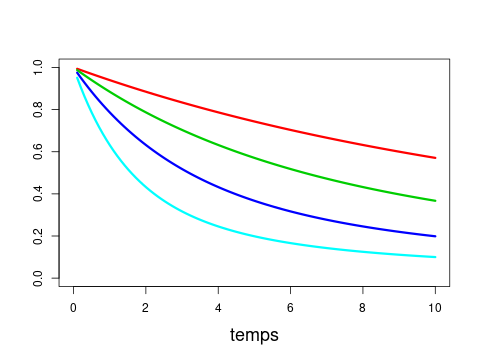
\includegraphics[width=0.5\textwidth, trim=20 40 20 50, clip=]{TumeurCDH1-ProbaApparition}
  $$
  }  
%   \begin{figure}
%     \begin{center}
%     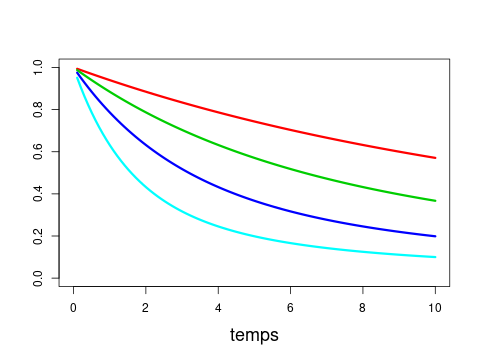
\includegraphics[width=0.5\textwidth, trim=20 40 20 50, clip=]{TumeurCDH1-ProbaApparition}
%     \caption{Probabilité $\phi(t)$ pour $\lambda = 1$ et \textcolor{red}{$\mu = 1/4$}, \textcolor{green}{$\mu = 1/2$} et \textcolor{blue}{$\mu = 1$}.}
%     \end{center}
%   \end{figure}
  %
\end{enumerate}

\bigskip
\paragraph{Loi du nombre de tumeurs de type M.}
On s'intéresse maintenant à la vitesse d'apparition des tumeurs de type M.

\bigskip
\begin{enumerate}
  \setcounter{enumi}{4}
  \item Donner la loi du nombre $M(t)$ de tumeurs de type M sachant le nombre total $N(t)$ de tumeurs apparues avant $t$ est égale à $n$: $N(t) = n$.
  \solution{
  Conditionnellement au fait que $n$ tumeurs sont apparues au temps $t$, chacune d'entre elle est encore de type B avec probabilité $\pi(t)$ et est donc de type M avec probabilité $1 - \pi(t)$. Ces tumeurs étant apparues et s'étant transformées indépendamment, le nombre de tumeurs de type M au temps $t$ suit une loi binomiale :
  $$
  \left(M(t) \mid N(t) = n\right) \sim \Bcal(n, 1 - \pi(t)).
  $$
  \paragraph{\sl Alternative.} On peut aussi reprendre le calcul de la question précédente en intégrant simultanément sur les temps d'apparition $s_1 \dots s_n$ des $n$ cellules présentes et en distinguant celles qui sont restées de type B (avec probabilité $e^{-\mu(t - s)}$) de celles qui se sont transformées en cellules de type M (avec probabilité $1 - e^{-\mu(t - s)}$). On écrit ainsi $\Pr\{M(t) = m \mid N(t) = n\}$
  \begin{align*}
    & = \idotsint_{[0, t]^n} \binom{n}{m} \prod_{j=1}^m \frac1t \underset{\text{passée en type M}}{\underbrace{(1- e^{-\mu(t-s_j)})}} \d s_j \prod_{k=m+1}^{n} \frac1t \underset{\text{toujours de type B}}{\underbrace{e^{-\mu(t-s_k)}}} \d s_k \\
    & = \binom{n}{m} \prod_{j=1}^m \left(\frac1t \int_{[0, t]} (1- e^{-\mu(t-s_j)}) \d s_j \right) \prod_{k=m+1}^{n} \left(\frac1t \int_{[0, t]} e^{-\mu(t-s_k)} \d s_k\right) \\
%     & = \binom{n}{m} \left(1 -e^{-\mu t} \left[\frac{e^{\mu t}-1}{\mu}\right]\right)^m  \left( e^{-\mu t} \left[\frac{e^{\mu t}-1}{\mu}\right]\right)^{n-m} \\
    &= \binom{n}{m} \left(1- \frac{1 - e^{-\mu t}}{\mu t}\right)^m \left( \frac{1 - e^{-\mu t}}{\mu t}\right)^{n-m}
  \end{align*}
  où on reconnait une loi binomiale :
  $$
  \left(M(t) \mid N(t) = n\right) \sim \Bcal(n, 1 - \pi(t)).
  $$
  }
  %
  \item En déduire la loi du nombre $M(t)$ de tumeurs de type M apparues avant $t$.
  \solution{
  On applique le résultat de la question préliminaire avec $X = N(t)$, $\alpha = \lambda t$, $Y = M(t)$ et $p = 1 - \pi(t)$ pour obtenir que le nombre de tumeurs de type M au temps $t$ suit une loi de Poisson :
  $$
  M(t) \sim \Pcal\left(\lambda t [1 - \pi(t)]\right).
  $$
  }
  %
  \item Donner la probabilité qu'aucune tumeur de type M ne soit apparue au temps $t$.
  \solution{
  Puisque la probabilité qu'une variable de Poisson de paramètre $m$ soit nulle vaut $e^{-m}$, on a 
  $$
  \Pr\{M(t) = 0\} 
  = \exp\left(- \lambda t [1 - \pi(t)]\right)
  = \exp\left(- \lambda \left[t - \frac{1 - e^{-\mu t}}{\mu}\right]\right)
  $$
  La figure suivante donne $\Pr\{M(t) = 0\}$ pour $\lambda = 1$ et \textcolor{red}{$\mu = 1/8$}, \textcolor{green}{$\mu = 1/4$}, \textcolor{blue}{$\mu = 1/2$} et \textcolor{cyan}{$\mu = 1$}. 
  La courbe noire donne la probabilité d'absence de toute tumeur : $\Pr\{N(t) = 0\} = e^{-\lambda t}$.
  $$
  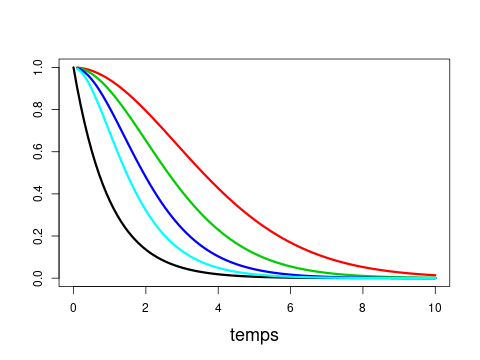
\includegraphics[width=0.5\textwidth, trim=20 40 20 50, clip=]{TumeurCDH1-ProbaAbsence}
  $$
  }
  %
  \item On suppose qu'en moyenne un tumeur bénigne apparaît chaque année ($\lambda = 1$) et que chacune d'elle devient maligne en moyenne au bout de cinq ans ($\mu = 1/5$). Calculer la probabilité qu'aucune tumeur maligne ne soit apparue au bout de $t = 10$ ans.
  \solution{
  Le paramètres sont alors $\lambda = 1$, $\mu = 1/5$ et $t = 10$, qui donne
  $\Pr\{M(t) = 0\} = 0.0034 = 0.34\%$.
  }
\end{enumerate}
